% Use the ijcai22 format

%%%% ijcai22.tex

\typeout{IJCAI--22 Instructions for Authors}

% These are the instructions for authors for IJCAI-22.

\documentclass{article}
\pdfpagewidth=8.5in
\pdfpageheight=11in
% The file ijcai22.sty is NOT the same as previous years'
\usepackage{ijcai22}

% Use the postscript times font!
\usepackage{times}
\usepackage{soul}
\usepackage{url}
\usepackage[hidelinks]{hyperref}
\usepackage[utf8]{inputenc}
\usepackage[small]{caption}
\usepackage{graphicx}
\usepackage{amsmath}
\usepackage{amsthm}
\usepackage{booktabs}
\usepackage{algorithm}
\usepackage{algorithmic}
\usepackage{tkz-graph}
\usepackage{caption}
\usepackage{subcaption}

\urlstyle{same}

% the following package is optional:
%\usepackage{latexsym}

% See https://www.overleaf.com/learn/latex/theorems_and_proofs
% for a nice explanation of how to define new theorems, but keep
% in mind that the amsthm package is already included in this
% template and that you must *not* alter the styling.
\newtheorem{example}{Example}
\newtheorem{theorem}{Theorem}

\newtheorem{definition}{Definition}
\newtheorem{proposition}{Proposition}

% Following comment is from ijcai97-submit.tex:
% The preparation of these files was supported by Schlumberger Palo Alto
% Research, AT\&T Bell Laboratories, and Morgan Kaufmann Publishers.
% Shirley Jowell, of Morgan Kaufmann Publishers, and Peter F.
% Patel-Schneider, of AT\&T Bell Laboratories collaborated on their
% preparation.

% These instructions can be modified and used in other conferences as long
% as credit to the authors and supporting agencies is retained, this notice
% is not changed, and further modification or reuse is not restricted.
% Neither Shirley Jowell nor Peter F. Patel-Schneider can be listed as
% contacts for providing assistance without their prior permission.

% To use for other conferences, change references to files and the
% conference appropriate and use other authors, contacts, publishers, and
% organizations.
% Also change the deadline and address for returning papers and the length and
% page charge instructions.
% Put where the files are available in the appropriate places.

% PDF Info Is REQUIRED.
% Please **do not** include Title and Author information
\pdfinfo{
	/TemplateVersion (IJCAI.2022.0)
}

\title{Bayesian Networks and Graph Rewrites}

% Single author syntax
\author{
	Adam Chen
	\affiliations
	Stevens Institute of Technology
	\emails
	achen19@stevens.edu
}

\newcommand{\problemone}{Same-Variable Equivalency Problem}
\newcommand{\problemtwo}{Different-Variable Equivalency Problem}


\begin{document}
	
	\maketitle
	
	\begin{abstract}
		It is known that Bayesian networks are an insufficient model for causality, as they merely describe the decomposition of a joint probability into conditional probabilities.
		This fails, in most cases, to capture directionality --- a crucial aspect of causality.
		Furthermore, conditional probability fails to tell us about hidden confounders.
		
		I look at the mathematical formalizations of these two shortcomings, and review the existing corpus of work on their categorization.
		I implement a tool to analyze when these shortcomings may be an issue and create ambiguities in Bayesian networks.
		The tool is used to find ambiguities in practical, real-life Bayesian networks, and the implications of such ambiguities on causal inference is discussed.
	\end{abstract}
	
		
	\section{Equivalent Bayesian Networks}
	\subsection{Background}
	A Bayesian network is a tuple of a directed acyclic graph (DAG) and a probability distribution over variables corresponding to the vertices of the DAG, such that the probability measure to be compatible with the DAG, defined thusly:
	\begin{definition}[Compatibility (Fong)\cite{fong2013causal}]
		Graph $G$ is compatible with probability measure (over the vertices of $G$) $P$, if
		$$
		P(x_1, \dots, x_n) = \prod_{i=1}^n{P(x_i \mid pa(x_i))}
		$$
		where $pa(x_i)$ is the parents of $x_i$ in $G$.
	\end{definition}
	For the remainder of the paper, I may use ``Bayesian network'' to refer to the DAG associated with a Bayesian network.
	
	\paragraph{Equivalency} Intuitively, two DAGs are equivalent when they are compatible with the same probability distributions. More formally:
	\begin{definition}[Equivalency (Chickering)\cite{chickering2013transformational}]
		$G$ is equivalent to $G'$ if $\forall P_G: (G, P_G)$ is a Bayesian network $\iff (G', P_G')$ is a Bayesian network.
	\end{definition}
	
	For a simple example of equivalent Bayesian networks, consider the DAG of two nodes $A \rightarrow B$. The underlying probability distribution satisfies:
	$$
	P(A, B) = P(A)*P(B \mid A) = \\
	P(A)*\frac{P(A \cap B)}{P(A)} = P(A \cap B)
	$$
	which is the exact same requirement for the graph of $A \leftarrow B$.
	Thus the two DAGs are equivalent.
%	$A \rightarrow B \rightarrow C$ is indistinguishable from $C \rightarrow B \rightarrow A$. However, substituting one structure with another in all cases may not preserve validity of a Bayesian network.
	
%	We may take a structure $A \rightarrow B$ and replace it with creating a new node $C$ with $A \leftarrow C \rightarrow B$.
	
	
	\subsection{Motivating Example}
	
	\begin{figure}[b]
		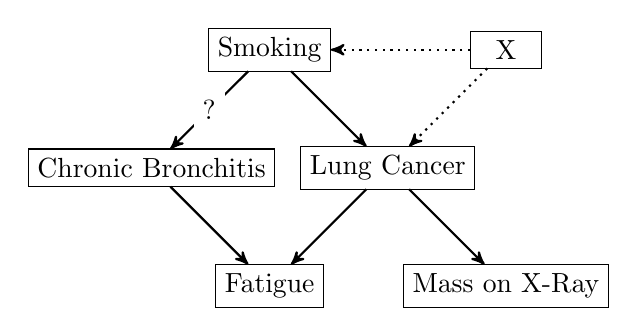
\begin{tikzpicture}[scale=1]
			\tikzstyle{VertexStyle} = [shape=rectangle,minimum width=6ex, draw]
			\tikzstyle{EdgeStyle}   = [->,>=stealth']
			
			\SetGraphUnit{1.5}
			\Vertex{Smoking}  \SOWE(Smoking){Chronic Bronchitis} \SOEA(Smoking){Lung Cancer}
			\SOEA(Chronic Bronchitis){Fatigue} \SOEA(Lung Cancer){Mass on X-Ray} \NOEA(Lung Cancer){X}
			\Edge[label=?](Smoking)(Chronic Bronchitis) \Edge(Smoking)(Lung Cancer)
			\Edge(Lung Cancer)(Fatigue) \Edge(Lung Cancer)(Mass on X-Ray) \Edge(Chronic Bronchitis)(Fatigue)
			\Edge[style=dotted](X)(Smoking) \Edge[style=dotted](X)(Lung Cancer)
		\end{tikzpicture}
		\caption{Example of a Bayesian network. Are we able to reverse the ``?'' arrow? Are we able to add the X node (and dotted edges)?}
		\label{dir-ex}
	\end{figure}
	
	Consider the Bayesian network shown in Figure \ref{dir-ex}, modified with two proposed changes from one presented in slides by Kleinberg\cite{lec4slides}.
	
	We know that in simple examples, as shown before, we may be able to reverse the direction of an arrow and have an equivalent Bayesian network.
	Is it the case that we can flip the arrow labeled with ``?'' and have an equivalent network? More generally, what are all of ways we can change the edges (be it flipping them, or removing and/or adding new edges) and have an equivalent network? I refer to this as the ``\problemone''. 

	We also know that many cases, there is some underlying cause (say X), that causes two other variables, thus creating an apparent correlation (in the example, smoking and lung cancer). In this example, can we add the node X and maintain compatibility with the joint probability distributions (excluding X) described by the original network? More generally, how can we add (or remove) nodes while maintaining compatibility on the restricted domain? I refer to this as the ``\problemtwo''.
	
	\subsection{Goals}
	In Sections \ref{problemone} and \ref{problemtwo}. I will formalize the two problems briefly described.
	Then, for each, I will present the theory for the resolution to the problems.
	The resolutions will be implemented as described in Section \ref{evaluation}, and the implementation will be used to evaluate several purported causal Bayesian networks to analyze the implicit assumptions.
	Finally, in Section \ref{discussion}, I discuss the implications of these problems on inferring causal relationships from observational data.


	\section{\problemone}
	\label{problemone}
	
	Verma \& Pearl\cite{verma2013equivalence} give a necessary and sufficient condition for testing the equivalence of Bayesian networks.
	Specifically, and phrased more simply by Chickering\cite{chickering2013transformational}, two Bayesian networks are equivalent if they have the same:
	\begin{enumerate}
		\item Skeleton: set of vertices and undirected edges.
		\item V-Structures: set of all unshielded colliders (i.e. triples of the form $X \rightarrow Y \leftarrow Z$ with $X$ not adjacent to $Z$).
	\end{enumerate}
	More generally, since each Bayesian network belongs to a finitely-sized equivalence class of networks completely determined by skeleton and v-structures, we may characterize all networks equivalent to a given network by those factors.
	
	Notably, since it is the case that equivalent networks must have the same skeleton, we may limit our consideration to only how we assign directions to the edges of a network, not changing the structure of the edges themselves.
	
	In the case of whether a single edge is reversible (while preserving equivalence), Chickering\cite{chickering2013transformational} presents a necessary and sufficient condition: the edge $X \rightarrow Y$ is reversible if and only if the parents of $Y$ are exactly $X$ and the parents of $X$.
	(Moreover, they show that every equivalent network may be reached by a sequence of such edge reversals.)
	
	\paragraph{Revisiting the Motivating Example}
	
	Recall Figure \ref{dir-ex}. Observe that the sole parent of the Chronic Bronchitis node is the Smoking node, and that the Smoking node has no parents.
	In other words, Chickering's condition is satisfied, so we may conclude that that edge is reversible.
	
	More generally, we may want to know what are \emph{all} the possible assignments of directions to arrows that maintain equivalency.
	To do so, we note that the only v-structure in the graph is Chronic Bronchitis $\rightarrow$ Fatigue $\leftarrow$ Lung Cancer.
	Thus we may erase the arrows on all other edges, and we obtain Figure \ref{undir-ex}.
	
	\begin{figure}[t]
	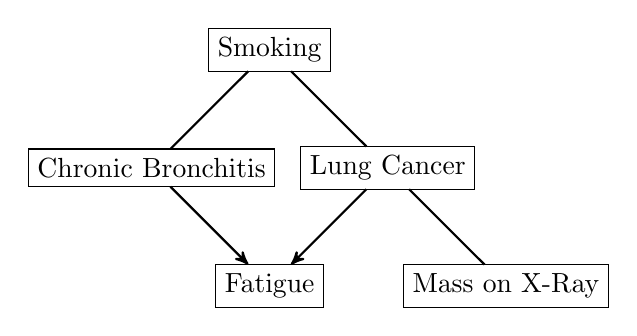
\begin{tikzpicture}[scale=1]
		\tikzstyle{VertexStyle} = [shape=rectangle,minimum width=6ex, draw]
		\tikzstyle{EdgeStyle}   = [-,>=stealth']
		
		\SetGraphUnit{1.5}
		\Vertex{Smoking}  \SOWE(Smoking){Chronic Bronchitis} \SOEA(Smoking){Lung Cancer}
		\SOEA(Chronic Bronchitis){Fatigue} \SOEA(Lung Cancer){Mass on X-Ray}
		\Edge(Smoking)(Chronic Bronchitis) \Edge(Smoking)(Lung Cancer)
		\draw[thick, ->,>=stealth'](Lung Cancer)--(Fatigue); \Edge(Lung Cancer)(Mass on X-Ray) \draw[thick, ->,>=stealth'](Chronic Bronchitis)--(Fatigue);
	\end{tikzpicture}
	\caption{Replacing every undirected edge with an edge in an arbitrary direction, without introducing any new v-structures, yields an equivalent Bayesian network.}
	\label{undir-ex}
	\end{figure}

	However, we may not assign directions to the undirected edges however we please ($2^3=8$ ways).
	The new assignment of directions must not introduce any new v-structures, and it must not create any cycles.
	These constraints limit the choice of direction to four options:
	\begin{enumerate}
		\item The graph as shown in Figure \ref{dir-ex}.
		\item Chronic Bronchitis $\rightarrow$ Smoking $\rightarrow$ Lung Cancer $\rightarrow$ Mass on X-Ray.
		\item Mass on X-Ray $\rightarrow$ Lung Cancer $\rightarrow$ Smoking $\rightarrow$ Chronic Bronchitis. \label{LCimpSmoking1}
		\item Chronic Bronchitis $\leftarrow$ Smoking $\leftarrow$ Lung Cancer $\rightarrow$ Mass on X-Ray. \label{LCimpSmoking2}
	\end{enumerate}
	Any other choice on arrows would create a new v-structure, either on (Chronic Bronchitis, Smoking, Lung Cancer), or on (Smoking, Lung Cancer, Mass on X-Ray). In this example, creating a cycle is impossible.
	
	\section{\problemtwo}
	\label{problemtwo}
	In Section \ref{problemone}, the case of changing the edge-structure of a DAG was investigated.
	Now, consider the cases where we change the number of nodes in a graph.
	On a practical level, node addition may be done if it is believed that an unmeasured variable is truly responsible for observed dependencies.
	Node removal may be done mostly for simplifying computation, but it may also be seen as the inverse process of node addition.
	That is, to ask the question of ``when can we add a node to a DAG'', it may be dually phrased as ``which DAGs yield this one once a node is removed''.
	
	Formally, we look at two forms of node removal: marginalization and conditioning.
	
	\paragraph{Node Removal}
	
	To give a semi-formal treatment of the problem statement, consider that we have measure (probability) spaces parameterized by each variable: $X_1, \dots, X_n$.
	Suppose we have a probability measure $P$ on the product space $X_1 \times \dots \times X_n$.
	We would like to, from this measure, derive a measure for the subspace $X_1 \times \dots \times X_{k-1} \times X_{k+1} \times \dots \times X_n$, essentially ``removing'' $X_k$.
	There are two canonical (and useful) ways to do so.
	Take $x_i \in X_i$:
	
	\begin{definition}[Marginalization (Barber)\cite{barberBRML2012}]
		The marginalization of probability measure $P(x_1, \dots, x_n)$ over $x_k$ is
		$$
		P(x_1,\dots,x_{k-1},x_{k+1},\dots,x_n) = \sum_{x_k}{P(x_1,\dots,x_n)}
		$$
	\end{definition}

	\begin{definition}[Conditioning]
		The conditioning of probability measure $P(x_1, \dots, x_n)$ on $x_k$ is
		$$
		P(x_1,\dots,x_{k-1},x_{k+1},\dots,x_n \mid x_k)$$
		$$ = \frac{P(x_1,\dots,x_n)}{P(x_k)}
		$$
	\end{definition}
	Note that the expression in the denomination is a marginalization.
	
	To see how these operations affect a Bayesian network, consider the simple examples of how parents and children of nodes are affected. Consider Figure \ref{commonparent}. Suppose we wanted the marginalization over A. By the Bayesian network, we know
	$$
	P(A, B, C) = P(A)P(B \mid A)P(C \mid A)
	$$
	$$
	\sum_A{P(A, B, C)} = \sum_A{P(A)P(B \mid A)P(C \mid A)}
	$$
	Which is not, in general, reducible to $P(B)P(C)$. Thus after marginalization, $B$ and $C$ are dependent, so there must be an edge between them. By contrast, consider the case in Figure \ref{collider}.
	$$
	P(A, B, C) = P(A \mid B, C)P(B)P(C)
	$$
	\[
	\begin{array}{ll}
	\sum_A{P(A, B, C)} & = \sum_A{P(A \mid B, C)P(B)P(C)} \\
					   & = P(B)P(C) \sum_A{P(A \mid B, C)} \\
					   & = P(B)P(C)
	\end{array}
	\]
	And so, $B$ and $C$ are independent and the Bayesian network after marginalization is the of $B$ and $C$ and no edges.
	
	In general, it appears that marginalization does not introduce new edges between parents. It appears to extend edges from each parent to each child, and create a directed clique among the children. I could not find a source proving this claim for DAGs in particular, but processes for variable elimination (marginalization) involve the moralization of the (undirected) hidden Markov model corresponding to the DAG\cite{kollerVarElim}.
	
	For simple cases of conditioning, we find the opposite effect as marginalization (very much suggesting that it is a dual process).
	Barber\cite{barberBRML2012} creates the same example graphs, and asserts that in Figure \ref{commonparent}, conditioning on A creates an edge between B and C, and in Figure \ref{collider}, conditioning on A results in a graph with no edges.
	More generally, the case of conditioning may be more well understood through the mechanism of d-separation.
	Recall that two nodes x and y are dependent conditioned on a node z (more generally a set of nodes) if z d-separates x and y.
	We can use this condition to ascertain the structure of the graph resulting from conditioning on a variable.
	In particular, removing a node z necessarily creates a dependency between every pair of nodes d-separated by z.
	
	Once again, I could not locate a source proving this result, so I leave it as an unproven conjecture: conditioning on a node z yields a Bayesian network whose DAG is the original DAG, but with an additional edge between each node d-separated by z (thus forming a directed clique).
	
	\begin{figure}
		\centering
		\begin{subfigure}{0.45\columnwidth}
			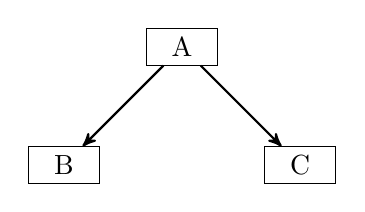
\begin{tikzpicture}[scale=1]
				\tikzstyle{VertexStyle} = [shape=rectangle,minimum width=6ex, draw]
				\tikzstyle{EdgeStyle}   = [->,>=stealth']
				
				\SetGraphUnit{1.5}
				\Vertex{A}  \SOWE(A){B} \SOEA(A){C}
				\Edge(A)(B) \Edge(A)(C)
			\end{tikzpicture}
			\subcaption{B and C conditioned on A.}
			\label{commonparent}
		\end{subfigure}
	\begin{subfigure}{0.45\columnwidth}
		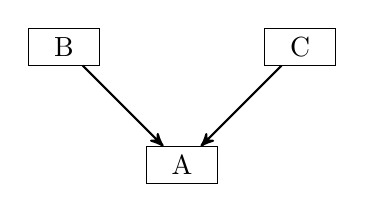
\begin{tikzpicture}[scale=1]
			\tikzstyle{VertexStyle} = [shape=rectangle,minimum width=6ex, draw]
			\tikzstyle{EdgeStyle}   = [->,>=stealth']
			
			\SetGraphUnit{1.5}
			\Vertex{A}  \NOWE(A){B} \NOEA(A){C}
			\Edge(B)(A) \Edge(C)(A)
		\end{tikzpicture}
		\subcaption{A conditioned on B and C.}
		\label{collider}
	\end{subfigure}
	\caption{DAGs illustrating the simplest non-trivial cases of parents and children.}
	\label{simple}
	\end{figure}

	\paragraph{Node Addition}
	
	I now arrive at the opposite problem, one that is more relevant to causal inference: the addition of new nodes.
	There is fundamental difficulty in that one cannot know a priori whether there is an underlying cause.
	First, allow me to semi-formally state the problem:
	
	Given a Bayesian network $(G, P)$, is it the case that:
	\[\begin{array}{l}
	\text{Characterize } (G',  P')\text{ such that: }\\
	\text{Vertices}(G') = \text{Vertices}(G') \cup \{x\} \wedge \\
	P \text{ is the marginalization/conditioning of } P' \text{ over/on x}.
	\end{array}\]
	
	where x is a node not in $G$. There are clearly trivial cases: marginalizing on leaves, conditioning on root nodes, and either operations on nodes whose variables have a trivial probability distribution (one outcome happens with probability 1).
	
	Since the problem is phrased in terms of the result of a node removal, operations that leave clear effects on the graph, we can look for such effects.
	Namely, they tend to form complete bipartite sub-graphs, and tend to form cliques.
	Elidan et. al\cite{elidanDiscovering2001} formalize this intuition; when such a Bayesian network is construct-able, then indeed, the probability measures satisfy the same independence constraints, and furthermore, the new graph is minimal (in some sense).
	
	The authors go on to describe that in inference contexts, the completely strict clique requirement is too much, and that semi-cliques are good indicators to try to infer hidden variables. They propose a heuristic-based algorithm for the detection of semi-cliques for the purposes of inference.
	
	\paragraph{Examples}
	Berkson's paradox is a well-known statistical paradox, where a sample skewed by thresholding admits an apparent (usually negative) correlation.
	It may be modeled in the realm of Bayesian networks by conditioning on a collider (e.g. conditioning on $A$ in Figure \ref{collider}).
	In the resulting observations, we see two variables that appear to be correlated, but in actuality are independent; a study's design may just be flawed in a way (apparent or not readily apparent) such that the conditioning occurs prior to data analysis.
	
	In the motivating example (ref. Figure \ref{dir-ex}), we wondered if a node X could be added above Smoking and Lung Cancer.
	It is clear that a trivial node could have been there --- either a node we condition on to get the graph we have currently, or a variable with a trivial probability distribution.
	The interesting case is whether there is an underlying cause (i.e. a node that we would marginalize on).
	As Smoking is a root node, there's no way to a priori (to collection of additional data) know whether there is an underlying cause; at the very least, in the view of Elidan et. al, the relative simplicity of the graph does not give us reason to believe that there should be one.
	
%	Inverse process? Data conditioned on something? Do math stuff and show trivial generalities. Berkson's paradox. Common cause.
%	In the case of inference, we may be more interested in whether our observed data is data marginalized on some hidden cause X.
	
%	marginalization as underlying causes, conditionalization as confounding (berkson's paradox)
	
%	Formally, is it the case that:
%	$$
%	\exists X: P(V_0, V_1, \dots, V_k) = \sum_X{P(V_0, V_1, \dots, V_k, X)}
%	$$
	
	
	
	\section{Evaluation}
	\label{evaluation}
	
	\subsection{Implementation}
	
	A program for reading in directed graphs (interpreted as Bayesian networks) and performing analyses on them was written.
	
	\paragraph{Bayesian Network Equivalence}
	As per the characterization of congruence classes of Bayesian networks presented in \cite{verma2013equivalence,chickering2013transformational}, testing for the equivalence of Bayesian networks was implemented via analysis on skeletons and v-structures.
	
	Additionally, a recursive, back-tracking assignment algorithm was implemented for enumerating \emph{all} Bayesian networks equivalent to a given network.
	Indeed, this tool was used to validate the explanation given for the motivating example.
	
	\paragraph{Node Removal/Addition}
	
	
	
	\subsection{Analysis of Other Bayesian Networks}
	
	Two other Bayesian networks from published papers were used to investigate the quality of causal networks in publications. \cite{Xu2018} \cite{liverDisorders}
	
	\subsection{Availability}
	The code for the tool, all example inputs and outputs, and the source for this paper are available on my GitHub at \url{https://github.com/Crazycolorz5/BayesianNetworkRewriting}.
	
	\section{Discussion}
	\label{discussion}
	
	It is known that Bayesian networks are, on their own, insufficient models of causality.
	Nevertheless, graphical models are useful for causal inference, and graphical models can capture many intuitions about causality (multiple causes, multiple effects, etc.).
	Thus when performing such inference, it is important to know how merely looking at dependence relations between data can lead us astray.
	
	More concretely, causal inference asserts several assumptions on top of pure statistical inference\cite{ramsey2012adjacencyfaithfulness}:
	\begin{itemize}
		\item The causal Markov condition: the set of variables has a causal structure that forms a DAG that satisfies the Bayesian conditional dependence rule.
		\item (Causal) faithfulness, decomposable as:
			\subitem Adjacency faithfulness: adjacent nodes are dependent given any combination of other nodes.
			\subitem Orientation faithfulness: when we have a v-structure (x, y, z), x and z are dependent given any subset of other nodes that contains y.
	\end{itemize}
	However, there are several problems.
	I have already shown that several distinct DAGs can be compatible with the same joint probability distribution.
	It is unclear that we can, a priori, know which DAG represents the proper causal structure.
	Indeed, Verma \& Pearl note that the recovery of a causal network from data is only up to modulo DAG equivalence\cite{verma2013equivalence}.
	It is also clear that the causal Markov condition (as presented) entails a form of completeness, e.g. common causes, which may appear as marginalized variables in a probabilistic network, are explicit.
	Once again, there appears to be no a priori way to know if all common causes are accounted for. I propose several suggestions to mitigate these problems, based on the findings in previous sections.
	
	\subsection{Measure Common Effects}
	The special importance of v-structures to the directness of a Bayesian network suggests that when designing a study, we should prioritize measuring variables that we believe will take this structure.
	Thus, the structure around these variables will be determined by the probability and so will not have an ambiguous direction.
	Namely, we would like to identify cases where there is a common effect (collider) of two independent causes (unshielded).
	
	As an example, suppose we wanted to argue that smoking (S) causes lung cancer (C).
	We know from the example in Figure \ref{undir-ex} that as drawn, we cannot (in the absence of outside information) determine whether it is smoking that plays a role in lung cancer, or vice versa.
	However, suppose we have another suspected cause of lung cancer, say asbestos exposure (A), and we believe that $S \perp A$.
	Then, in observation, we may find that $P(S, C, A) = P(S)*P(C \mid S, A)*P(A)$, and thus we know that the direction of those edges are forced.
	Then if we assume causal faithfulness, which one must to perform reasonable causal inference anyway, then we find that it must be the case that smoking causes lung cancer, not vice-versa.
	
	\subsection{The Importance of Ground Truth}
	An independent source of directionality can drastically narrow down the number of possible equivalent Bayesian networks. For example, in the motivating example, if we know externally that Smoking $\rightarrow$ Lung Cancer, we can eliminate options (\ref{LCimpSmoking1}) and (\ref{LCimpSmoking2}), as they do not obey this direction.
	Considering that the theoretical ceiling on direction assignments is $2^n$, where $n$ is the number of undirected edges, it is possible that each ground truth (that is not already implied by the v-structures) can reduce the possibility space exponentially.
	
	\subsection{Underlying Causes}
	
	\bibliographystyle{plain}
	\bibliography{references}
	
	\appendix
	
\end{document}
